%!TEX program = xelatex
% 完整编译: xelatex -> biber/bibtex -> xelatex -> xelatex
\documentclass[lang=cn,a4paper,newtx]{elegantpaper}

\title{A2赛题: 软件功能需求分析报告}
\author{荀阳霖	\\ 韶关学院 \and 程家骏 \\ 华中科技大学 \and 刘思辰\\ 华中科技大学 \and 龚言龙 \\ 华中科技大学}
\institute{\href{https://elegantlatex.org/}{porter项目组}}

\version{1.0}
\date{\zhdate{2023/7/5}}

% 本文档命令
\usepackage{array}
\newcommand{\ccr}[1]{\makecell{{\color{#1}\rule{1cm}{1cm}}}}
\addbibresource[location=local]{reference.bib} % 参考文献,不要删除

\begin{document}

\maketitle

\begin{abstract}
    雷鸟是一个免费的邮件应用程序,可以方便地进行日程的管理,邮件的发送,thunderbird78相比与之前的版本增加了一些新的功能,如内置电子邮件加密和数字签名的功能等。
为loongarch架构移植thunderbird78或者以上版本可以帮助丰富loongarch架构的生态,提高用户的使用体验。
\keywords{loongarch, thunderbird, 软件移植}
\end{abstract}

\section{任务介绍}

A2的赛题主要任务是为loongarch架构的桌面系统上移植thunderbird78或者以上的版本,并将其打包为deb包。
\subsection{所移植thunderbird信息}
Mozilla Thunderbird,非正式中文名称为雷鸟,是由Mozilla基金会研发的一款自由及开放源码的跨平台电邮客户端、新闻阅读器、聚合器以及即时通讯软件。


本次移植的雷鸟版本为114.0b6,由mozilla公司在7.27日进行发布,具体信息如图\ref{thunderbird}所示
\begin{figure}[!htb]
    \centering
    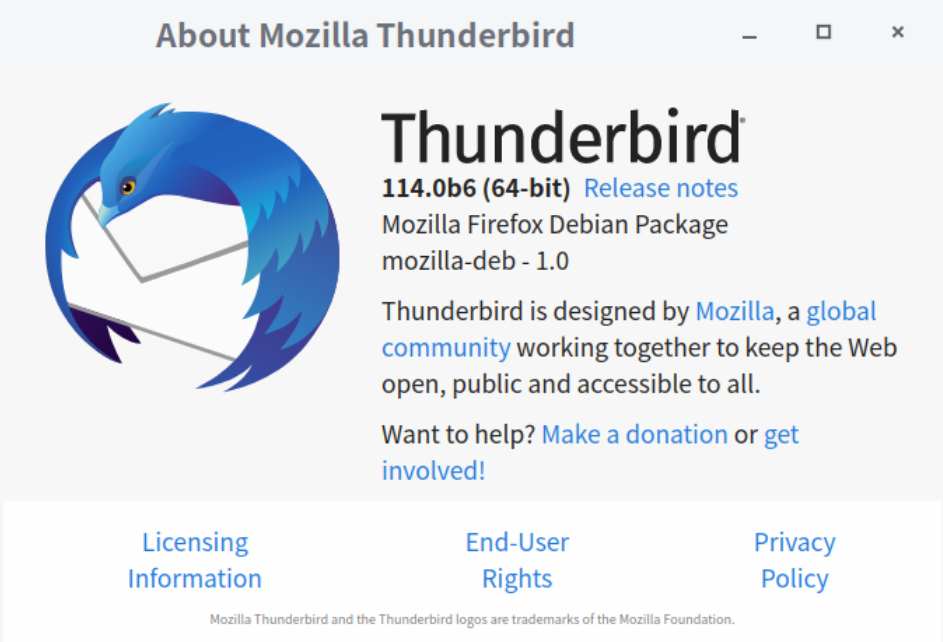
\includegraphics[width=0.6\textwidth]{thunderbird.png}
    \caption{开发机中thunderbird信息}
    \label{thunderbird}
\end{figure}

\subsection{功能需求}
\begin{enumerate}
    \item 能够在loongarch架构的机器上正常运行
    \item 通过testing目录下的测试样例
    \item 版本信息应该在78或者以上
\end{enumerate}
\subsection{开发环境}

loongnix操作系统,cpu型号3C5000L, cpu核数4核,4G内存,100G硬盘,进行fetch后得到的系统信息如图\ref{neofetch} 所示。

\begin{figure}[!htb]
    \centering
    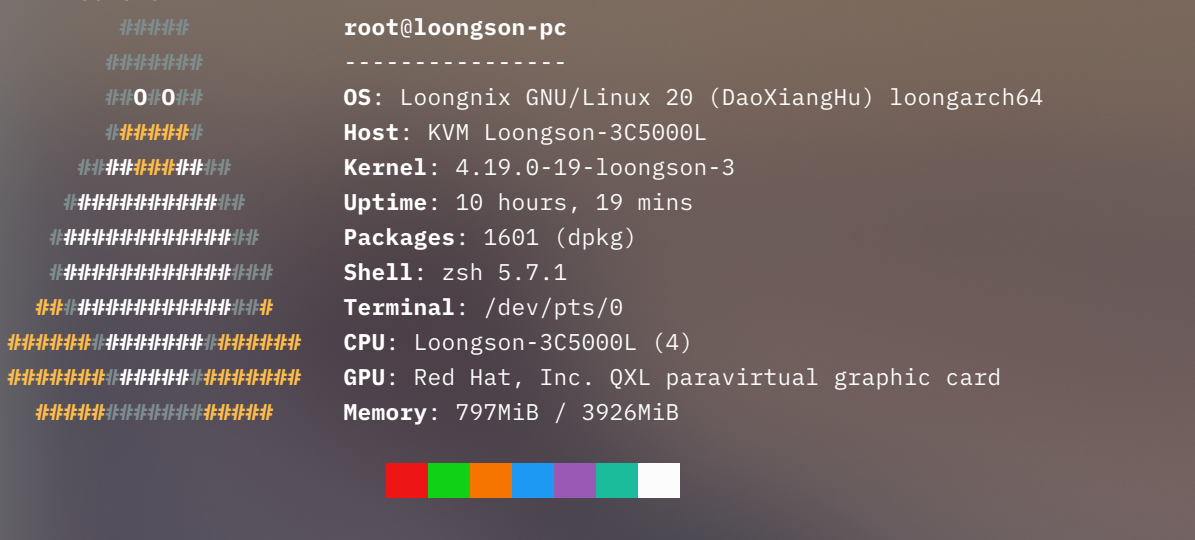
\includegraphics[width=0.8\textwidth]{fetch.png}
    \caption{neofetch结果}
    \label{neofetch}
\end{figure}


\section{软件移植记录}
\subsection{依赖适配}

编译thunderbird114及运行测试依赖于rustc1.69以上, 以及gcc13以上的版本,llvm13.0 以上的版本,因此我们在开发机上重新编译了相关的依赖,并同时将其中部分软件打包为deb包。

\subsubsection{rustc1.71.0-dev移植}
Loongarch已于24日进入Tier2。从5-25日开始,原版的rustup将提供nightly版的原生Loongarch rust工具链。从rust1.71开始,rustup将提供stable版本的原生Loongarch rust工具链

但是由于loongarch新旧世界的问题,无法直接使用最新的rust,需要在主机上进行交叉编译。

从rust仓库克隆1.71.0-dev到本地后,修改config.toml(修改可以参考如下所示),使得产出loongarch架构的二进制包。

\begin{lstlisting}
    changelog-seen = 2
    [build]
    docs = false
    host = ["loongarch64-unknown-linux-gnu"]
    target = ["loongarch64-unknown-linux-gnu","x86_64-unknown-linux-gnu"] #后面那个可以去掉

    #从2023年5月25日开始,很可能不需要用夜版来bootstrap了,但我没试过
    rustc = "/home/coa/.rustup/toolchains/nightly-x86_64-unknown-linux-gnu/bin/rustc"
    cargo = "/home/coa/.rustup/toolchains/nightly-x86_64-unknown-linux-gnu/bin/cargo"
    rustfmt = "/home/coa/.rustup/toolchains/nightly-x86_64-unknown-linux-gnu/bin/rustfmt"

    build-stage = 2

    # Enable a build of the extended Rust tool set which is not only the compiler
    # but also tools such as Cargo. 
    extended = true
    # Turn this off if you just want rustc -- CoA
    tools = [    
    "cargo"
    ]

    [target.loongarch64-unknown-linux-gnu]  # Change this if you need. (obviously) -- CoA
    cc = "/home/coa/CROSS/opt/cross/bin/loongarch64-unknown-linux-gnu-gcc"
    cxx = "/home/coa/CROSS/opt/cross/bin/loongarch64-unknown-linux-gnu-g++"
    ar = "/home/coa/CROSS/opt/cross/bin/loongarch64-unknown-linux-gnu-ar"
    ranlib = "/home/coa/CROSS/opt/cross/bin/loongarch64-unknown-linux-gnu-ranlib"
    linker = "/home/coa/CROSS/opt/cross/bin/loongarch64-unknown-linux-gnu-gcc"

    [rust]
    dist-src = false
    channel = "beta"

    [llvm]
    download-ci-llvm = false
    ccache = true  # 除非你确信真的只需要编译一次,将来也不打算换个rustc版本再试。否则最好还是保持打开的好
    targets = "LoongArch;X86"  # This will save a lot of time   -- CoA
    experimental-targets = ""  

    [dist]
    src-tarball = false
    compression-formats = ["xz"]
\end{lstlisting}

尽管loongnix的仓库中提供了loongnix1.65的rust,但是经过对比发现主线中的rust增加了对于loongarch的特定优化。

\subsubsection{gcc-13 移植}

gcc-13的移植较为顺利,从debian sid的源中直接获取到gcc-13deb包的源码包后,修改源码包中的debian/rules


在其中仅保留对c, c++语言的支持,同时关闭对32位的支持,如果开启对其他语言的支持,
将需要编译deb中的libffi,但是其中的libffi的版本为3.4.1,尚未引入对于loongarch架构的支持,3.4.3中引入了对于loongarch架构的支持,但是其需要的autoconf2.71,与gcc-13所需求的的2.69相互冲突,
所以我们最终选择进行关闭。

在编译雷鸟的过程中,仅开启对于c, c++的支持即可完成编译,

进行打包后生成的相关deb包如图\ref{deb}所示,如有需要欢迎联系chengjiajun20@gmail.com

\begin{figure}[!htb]
    \centering
    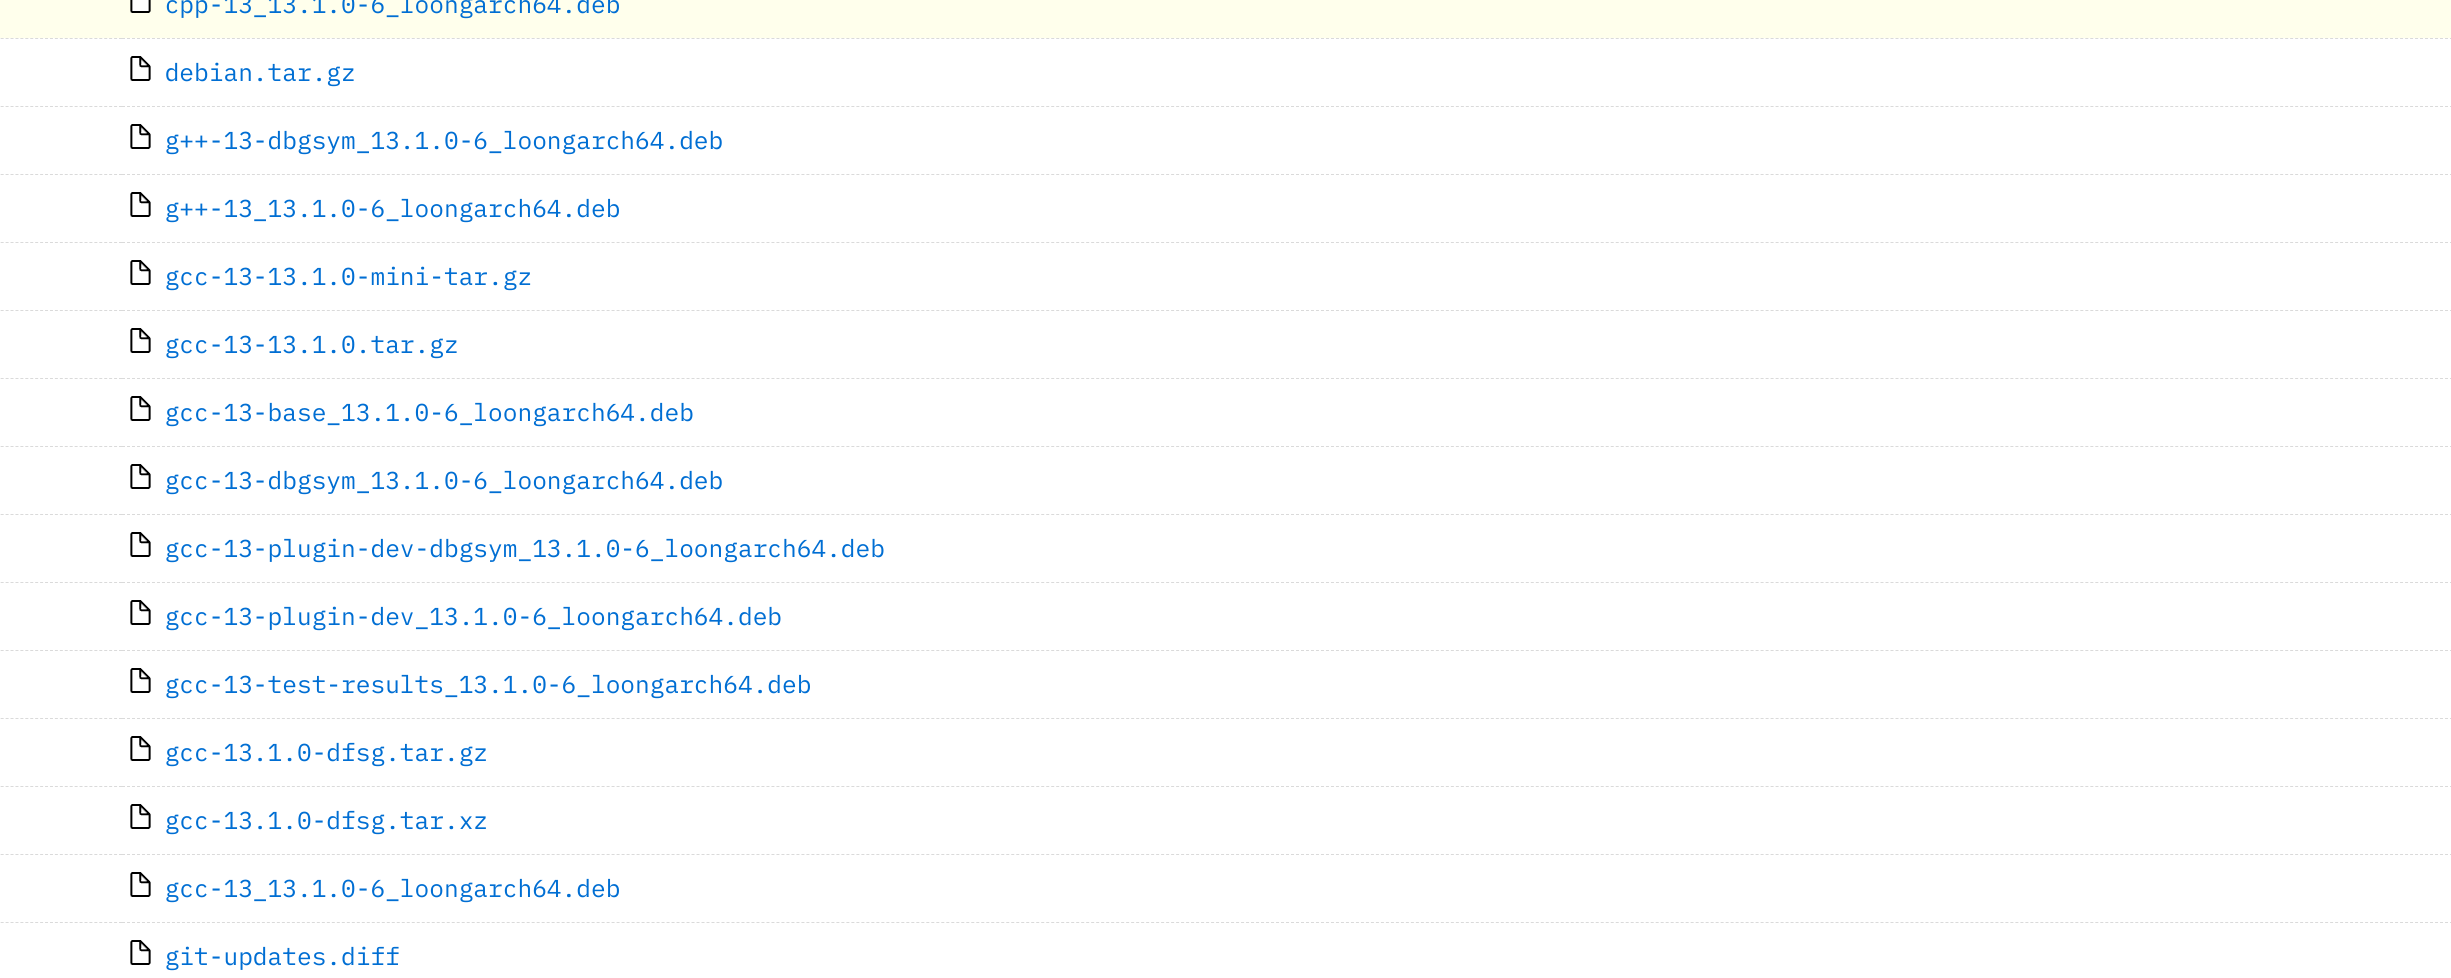
\includegraphics[width=1.0\textwidth]{package.png}
    \caption{生成的deb包}
    \label{deb}
\end{figure}

\subsubsection{llvm16.4移植}

当我们移植了gcc-13到本地之后,llvm的编译工作十分简单,只需要将llvm克隆到本地后进行编译即可。

\subsection{雷鸟打包}

修改雷鸟配置文件如下所示
\begin{lstlisting} 
    ac_add_options --enable-application=comm/mail
    ac_add_options --disable-crashreporter
    ac_add_options --without-wasm-sandboxed-libraries
    ac_add_options --enable-official-branding
    export MOZILLA_OFFICIAL=1
\end{lstlisting}

随后使用thunderbird和loongarch相关的patch,随后使用mach build进行编译,对于相关patch的解释如下所示

\begin{center}
    \begin{tabular}{cccc}
        \toprule
        patch & 来源 & 用途 & 潜在的问题\\
        \midrule
        &  &  & \\
        &  &  & \\
        \bottomrule
    \end{tabular}
\end{center}

修改python/mozbuild/mozbuild/repackaging/deb.py 在\_DEB\_ARCH中增加loongarch64的相关信息

\begin{lstlisting}
    _DEB_ARCH = {
            "all": "all",
            "x86": "i386",
            "x86_64": "amd64",
            "loongarch": "loongarch64"
        }
\end{lstlisting}

同时修改browser/installer/linux/debian内和rules相关的信息
\begin{enumerate}
    \item install.in 把 firefox 修改成 thunderbird
    \item links.in 把 firefox 修改成 thunderbird
\end{enumerate}

\section{软件使用}

如果需要使用我们的移植的thunderbird-114,那么此时需要将我们上传的
thunderbird-114.0b6.source.tar.xz以及thunderbird-default\_114.0~build1\_all.deb放入到deb软件源中
的对应位置。

如果您使用的dak等软件源搭建工具,进行合理的配置后将可以使得其进行自动的数据更新。
\section{致谢}

感谢LA UOSC社区对我们相关问题的回应,以及debian中文社区对deb打包相关问题的回复。


\nocite{*}
\printbibliography[heading=bibintoc, title=\ebibname]

\appendix
%\appendixpage
\addappheadtotoc

\end{document}
